\subsection{Čvorovi izraza}
\label{subsec:MyASTExpressionNodes}

Izraz, kao što se može videti na primeru gramatike sa slike \ref{fig:ANTLRExpressions}, se definiše rekurzivno i izraze mogu proširiti razni operatori. Na slici \ref{fig:ExpressionNodes} se mogu videti tipovi apstraktnih konstrukcija koje će se koristiti da bi se predstavili izrazi. Dodatno, za vezivanje izraza će se koristiti apstrakcije operatora definisane u prethodnom odeljku.

\begin{figure}[h!]
\centering
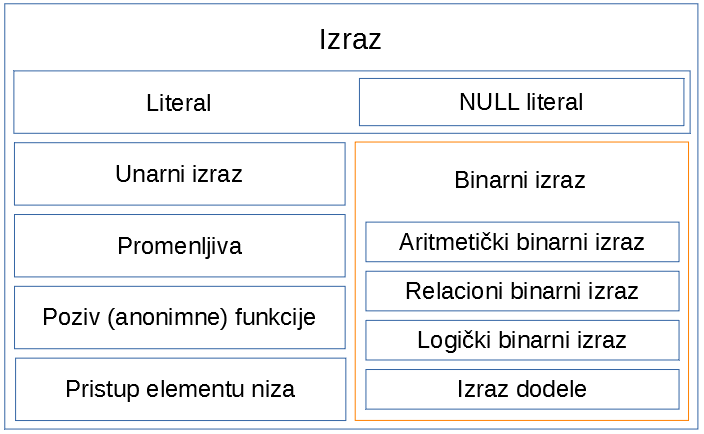
\includegraphics[scale=0.5]{images/expression_nodes.png}
\caption{Vrste čvorova izraza.}
\label{fig:ExpressionNodes}
\end{figure}

Najjednostavniji izraz predstavljaju konstante ili \emph{literali}. Literali mogu biti brojevne konstante, karakterske konstante ili konstantne niske. Literali često mogu imati i sufiks (najčešće za brojevne literale), koji određuje tip literala u slučajevima gde postoji dvosmislenost. Na primer, literal $5$ možemo posmatrati kao 32-bitni ceo broj ili kao 64-bitni ceo broj (ali i kao realan broj, ako ne zahtevamo da realne brojeve moramo pisati u nepokretnom ili pokretnom zarezu). Da bi se ova dvosmislenost uklonila, možemo eksplicitno naznačiti da se govori o 64-bitnom celom broju dodavanjem sufiksa \texttt{L}, ako je u pitanju programski jezik C ili njemu slični jezici. Takođe, pošto većina programskih jezika dozvoljava rad sa pokazivačima ili neposredno koristi alokaciju memorije za kreiranje objekata, uobičajeno je korišćenje prazne adrese kao specijalne vrednosti (\texttt{null} ili \texttt{nil}). Za ovu specijalnu vrednost je moguće kreirati poseban tip literala, jer ovaj literal može biti bilo kog tipa koji nije primitivni tip.

Osim literala, samostalne promenljive mogu predstavljati validan izraz, u kom slučaju je vrednost izraza trenutna vrednost te promenljive. Slično važi i za indeksni pristup nizu\footnote{Isto važi i za bilo koju drugu kolekciju, ukoliko je nad njom definisan operator indeksnog pristupa, predefinisanje ovog operatora nije razmatrano u ovom radu.}. U slučaju indeksnog pristupa, potrebno je navesti izraz čija vrednost označava indeks (to ne mora biti jednostavni literal). Postoje smislena ograničenja šta sve sme da se nađe unutar izraza koji predstavlja indeks elementa niza tako da to semantički ima smisla, ali se na ovom nivou ne bavimo semantičkom analizom. 

Unutar izraza se mogu naći i pozivi funkcija. Naravno, pretpostavljamo da funkcija ima povratnu vrednost, koja će se iskoristiti nakon poziva funkcije u kontekstu iz kojeg je ona pozvana. Pod uticajem funkcionalne paradigme, veliki broj programskih jezika dozvoljava definisanje anonimnih (lambda) funkcija, čija se definicija može smatrati izrazom koji se može dodeliti nekom simbolu. Stoga se i anonimne funkcije mogu smatrati validnim izrazima. 

Operatori opisani u \ref{subsec:MyASTOperatorNodes} mogu vezati sve tipove iznad i formirati složenije izraze. U zavisnosti od broja izraza koje operator vezuje, izraze možemo podeliti na unarne i binarne. Unarne izraze nadograđuju unarni operatori dok su binarni izrazi dobijeni primenom binarnog operatora na dva izraza. U zavisnosti od tipa binarnog operatora (videti sliku \ref{fig:OperatorNodes}), binarne izraze delimo na sličan način. Naravno, svaki od tipova binarnog izraza zahteva odgovarajući tip binarnog operatora. Slično se može uraditi i za unarne izraze, ali takođe i napraviti podela na prefiksne i postfiksne, ali to nije rađeno u ovom radu zarad pojednostavljenja --- u nekim jezicima su određeni operatori prefiksni dok su u drugim jezicima ti isti operatori postfiksni pa stoga nije pravljena ova podela.

Na slici \ref{fig:MyASTExampleExpressions} se mogu videti kreirani AST za izraz \texttt{(3 + 5) << f(4)}. Ovaj izraz poprima isti oblik bez obzira na to koji je programski jezik u pitanju, ali iako se sintaksa bude razlikovala ili operatori budu imali drugi simbol, logika operatora opisana putem funkcije će ostati ista.

\begin{figure}[h!]
\centering
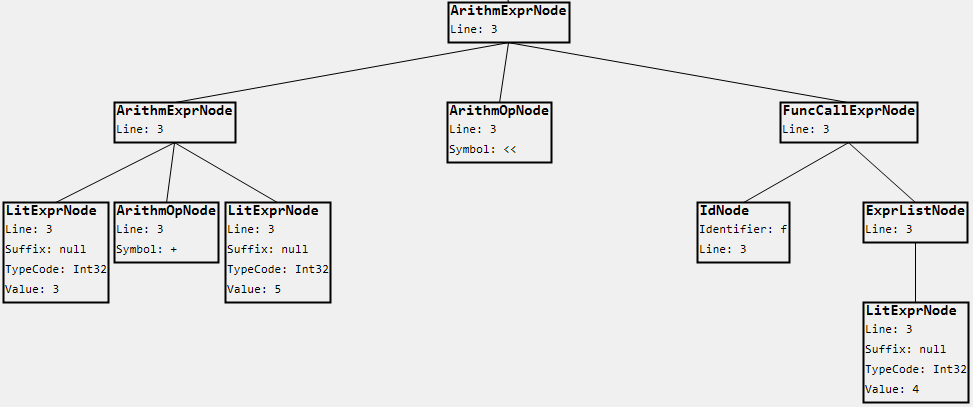
\includegraphics[scale=0.6]{images/ast_expr.png}
\caption{AST generisan od izraza \texttt{(3 + 5) << f(4)}.}
\label{fig:MyASTExampleExpressions}
\end{figure}
